The RSA algorithm is named after Ron \textbf{Rivest}, Adi \textbf{Shamir} and Len \textbf{Adleman}
who invented it in 1977, see~\cite{rivest1978method}.
The basic technique was first discovered in 1973 by Clifford Cocks~\cite{cocks1973note} of
CESG (part of the British GCHQ)
but this was a secret until 1997.
The patent taken out by RSA Labs has expired.

Historically, the process of encryption is considered to be symmetric one.
\begin{quote}
    \textbf{Symmetric encryption} -- is a type of encryption where only one secret key is
    used to both encrypt and decrypt information.
\end{quote}
It means that prior the communication the sides must conclude and share the secret key to be used in
both encryption and decryption.
Such approach is highly cost since it requires to share the defined secret keys between each actor.

\begin{figure}[H]
    \centering
    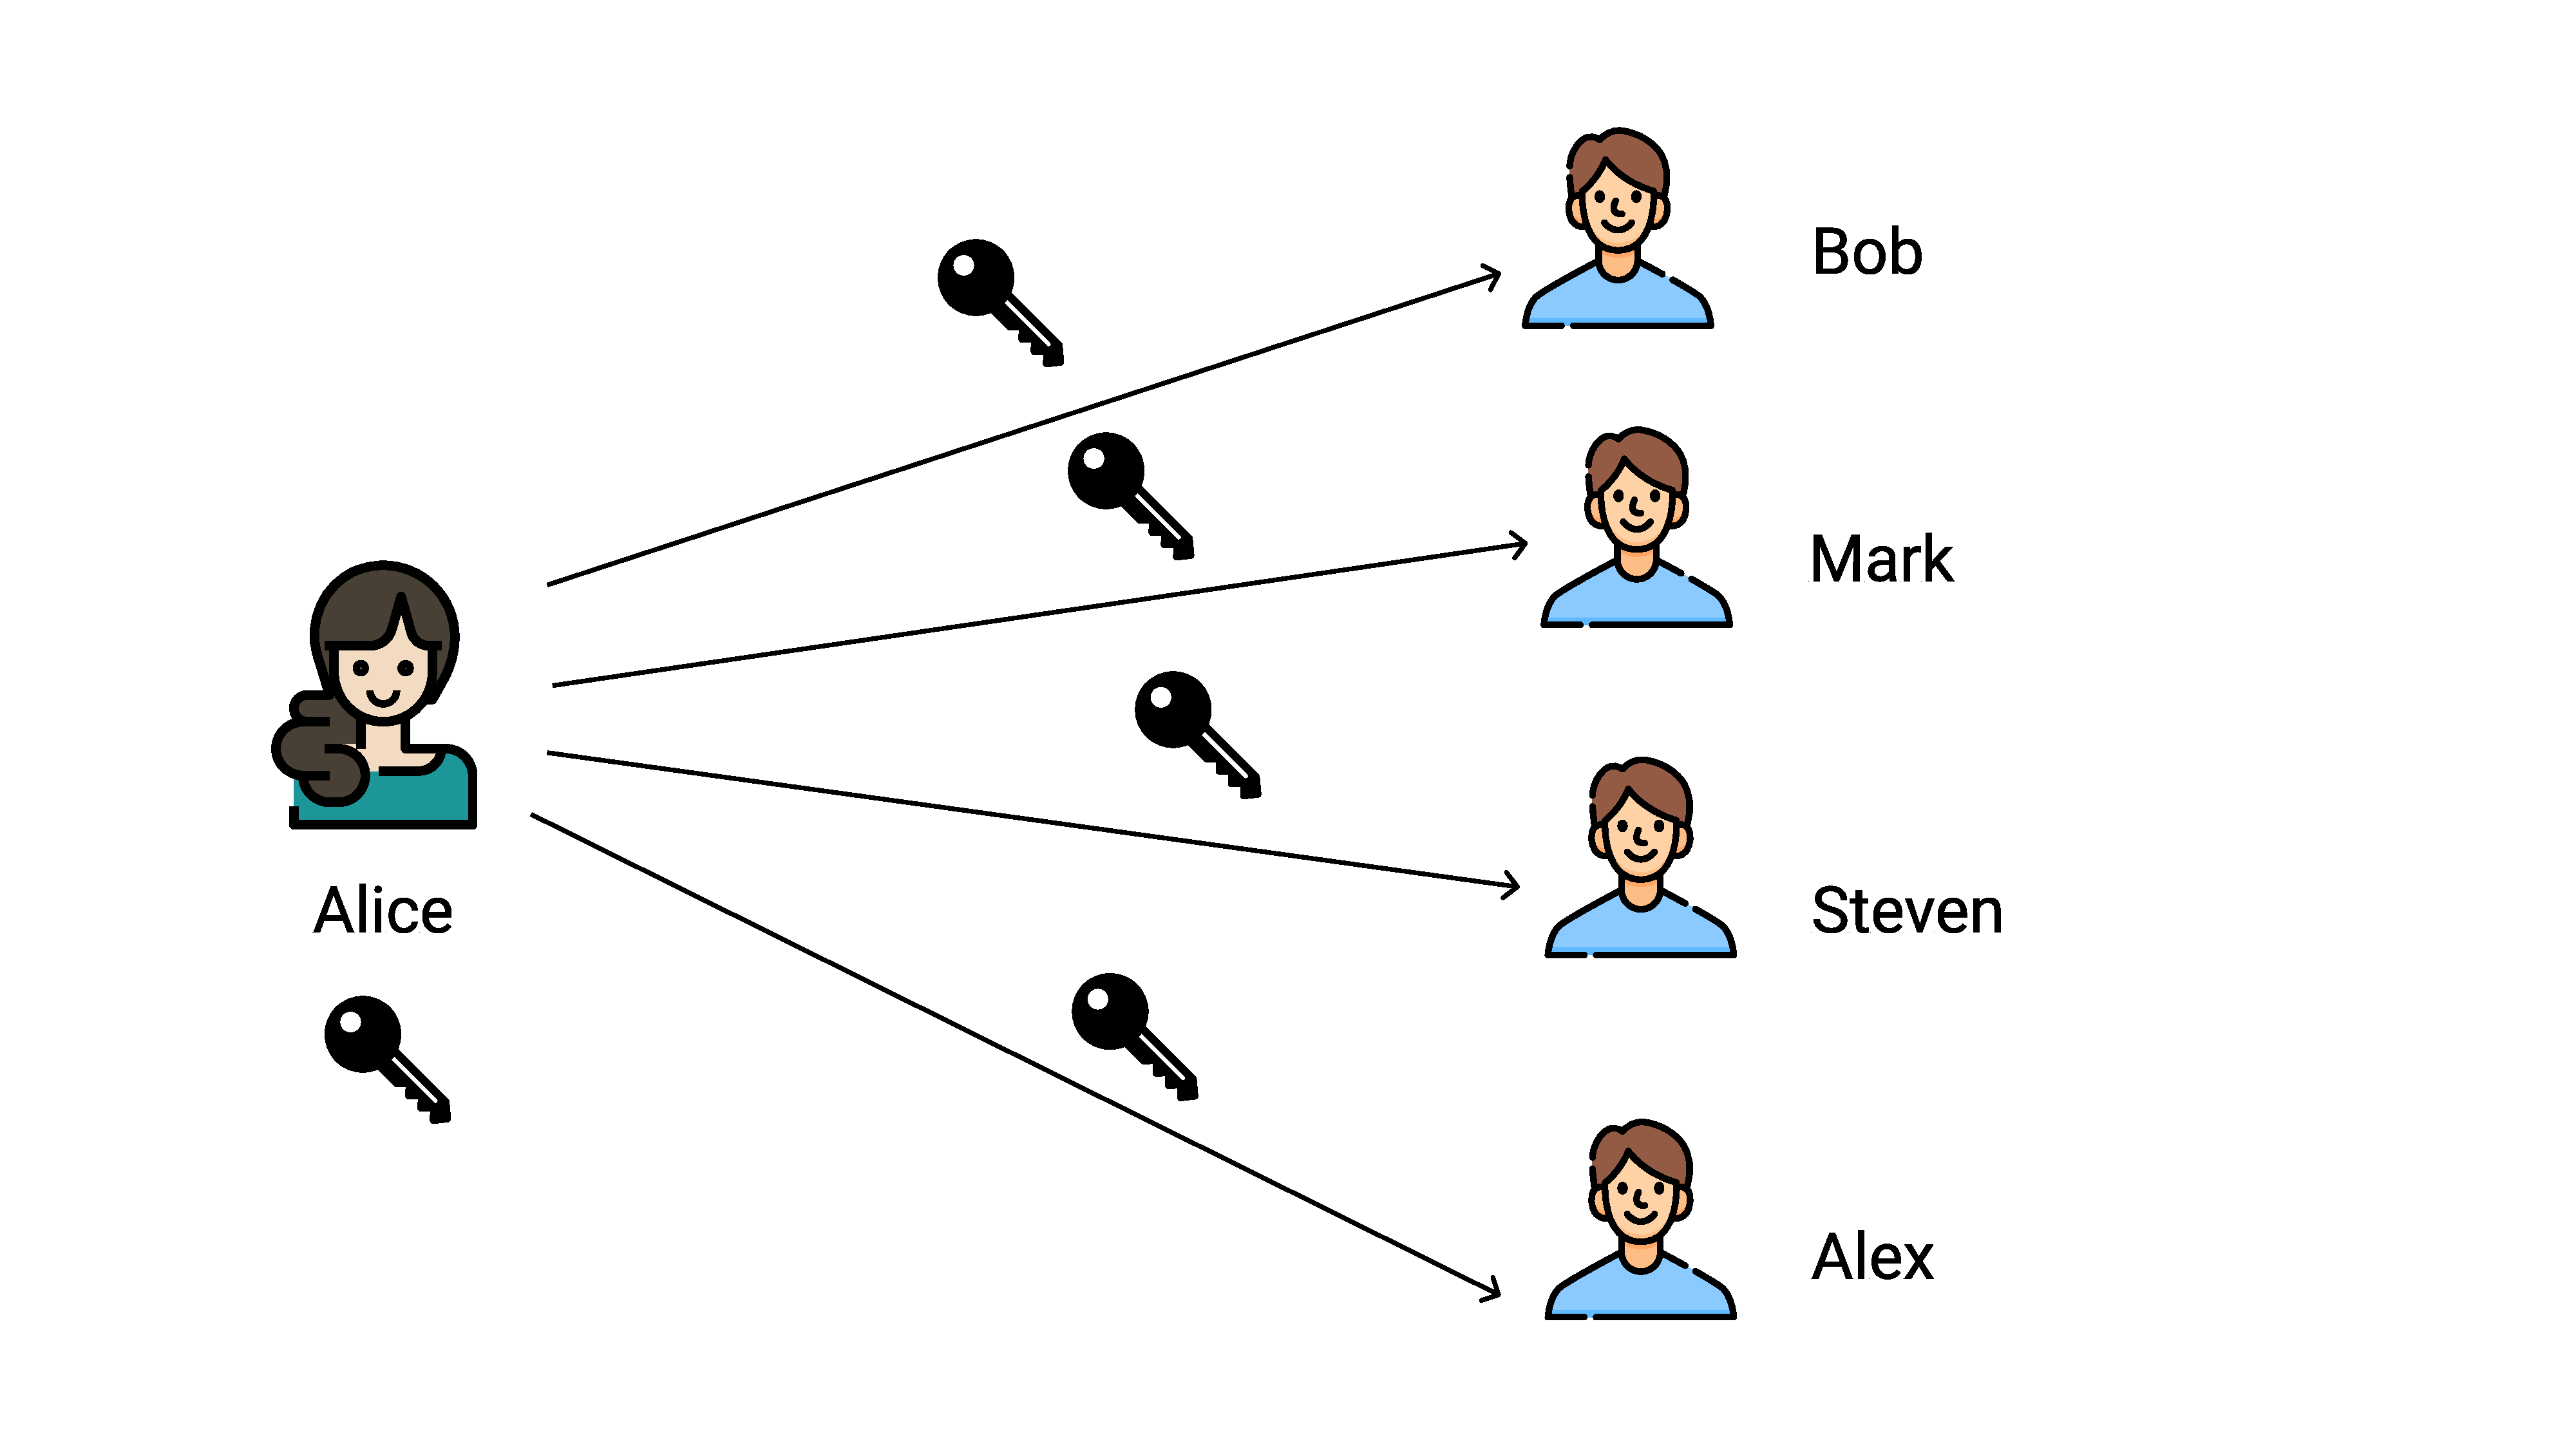
\includegraphics[width=1.15\textwidth]{img/Symmetric_encryption}
    ~\caption{Symmetric encryption real life example.}
    \label{fig:symmetric-encryption}
\end{figure}

The problem here is that Alice, Bob, Mark, Steven and Alex must exchange the secret keys securely,
for instance by means of Diffie-Hellman key exchange.

Much more simpler is to think about secured communication channel that in terms of asymmetric encryption.
\begin{quote}
    \textbf{Asymmetric encryption} -- is an encryption such that a message is encrypted using public key and
    decrypted using private key.
\end{quote}
Real life example would be if Alice shares with all the actors not the secret key, but \textbf{opened lock}.
Still Alice keeps the secret \textbf{private key} with herself,
but now she doesn't worry that intermediate eavesdropper would read her precious messages.
\begin{figure}[H]
    \centering
    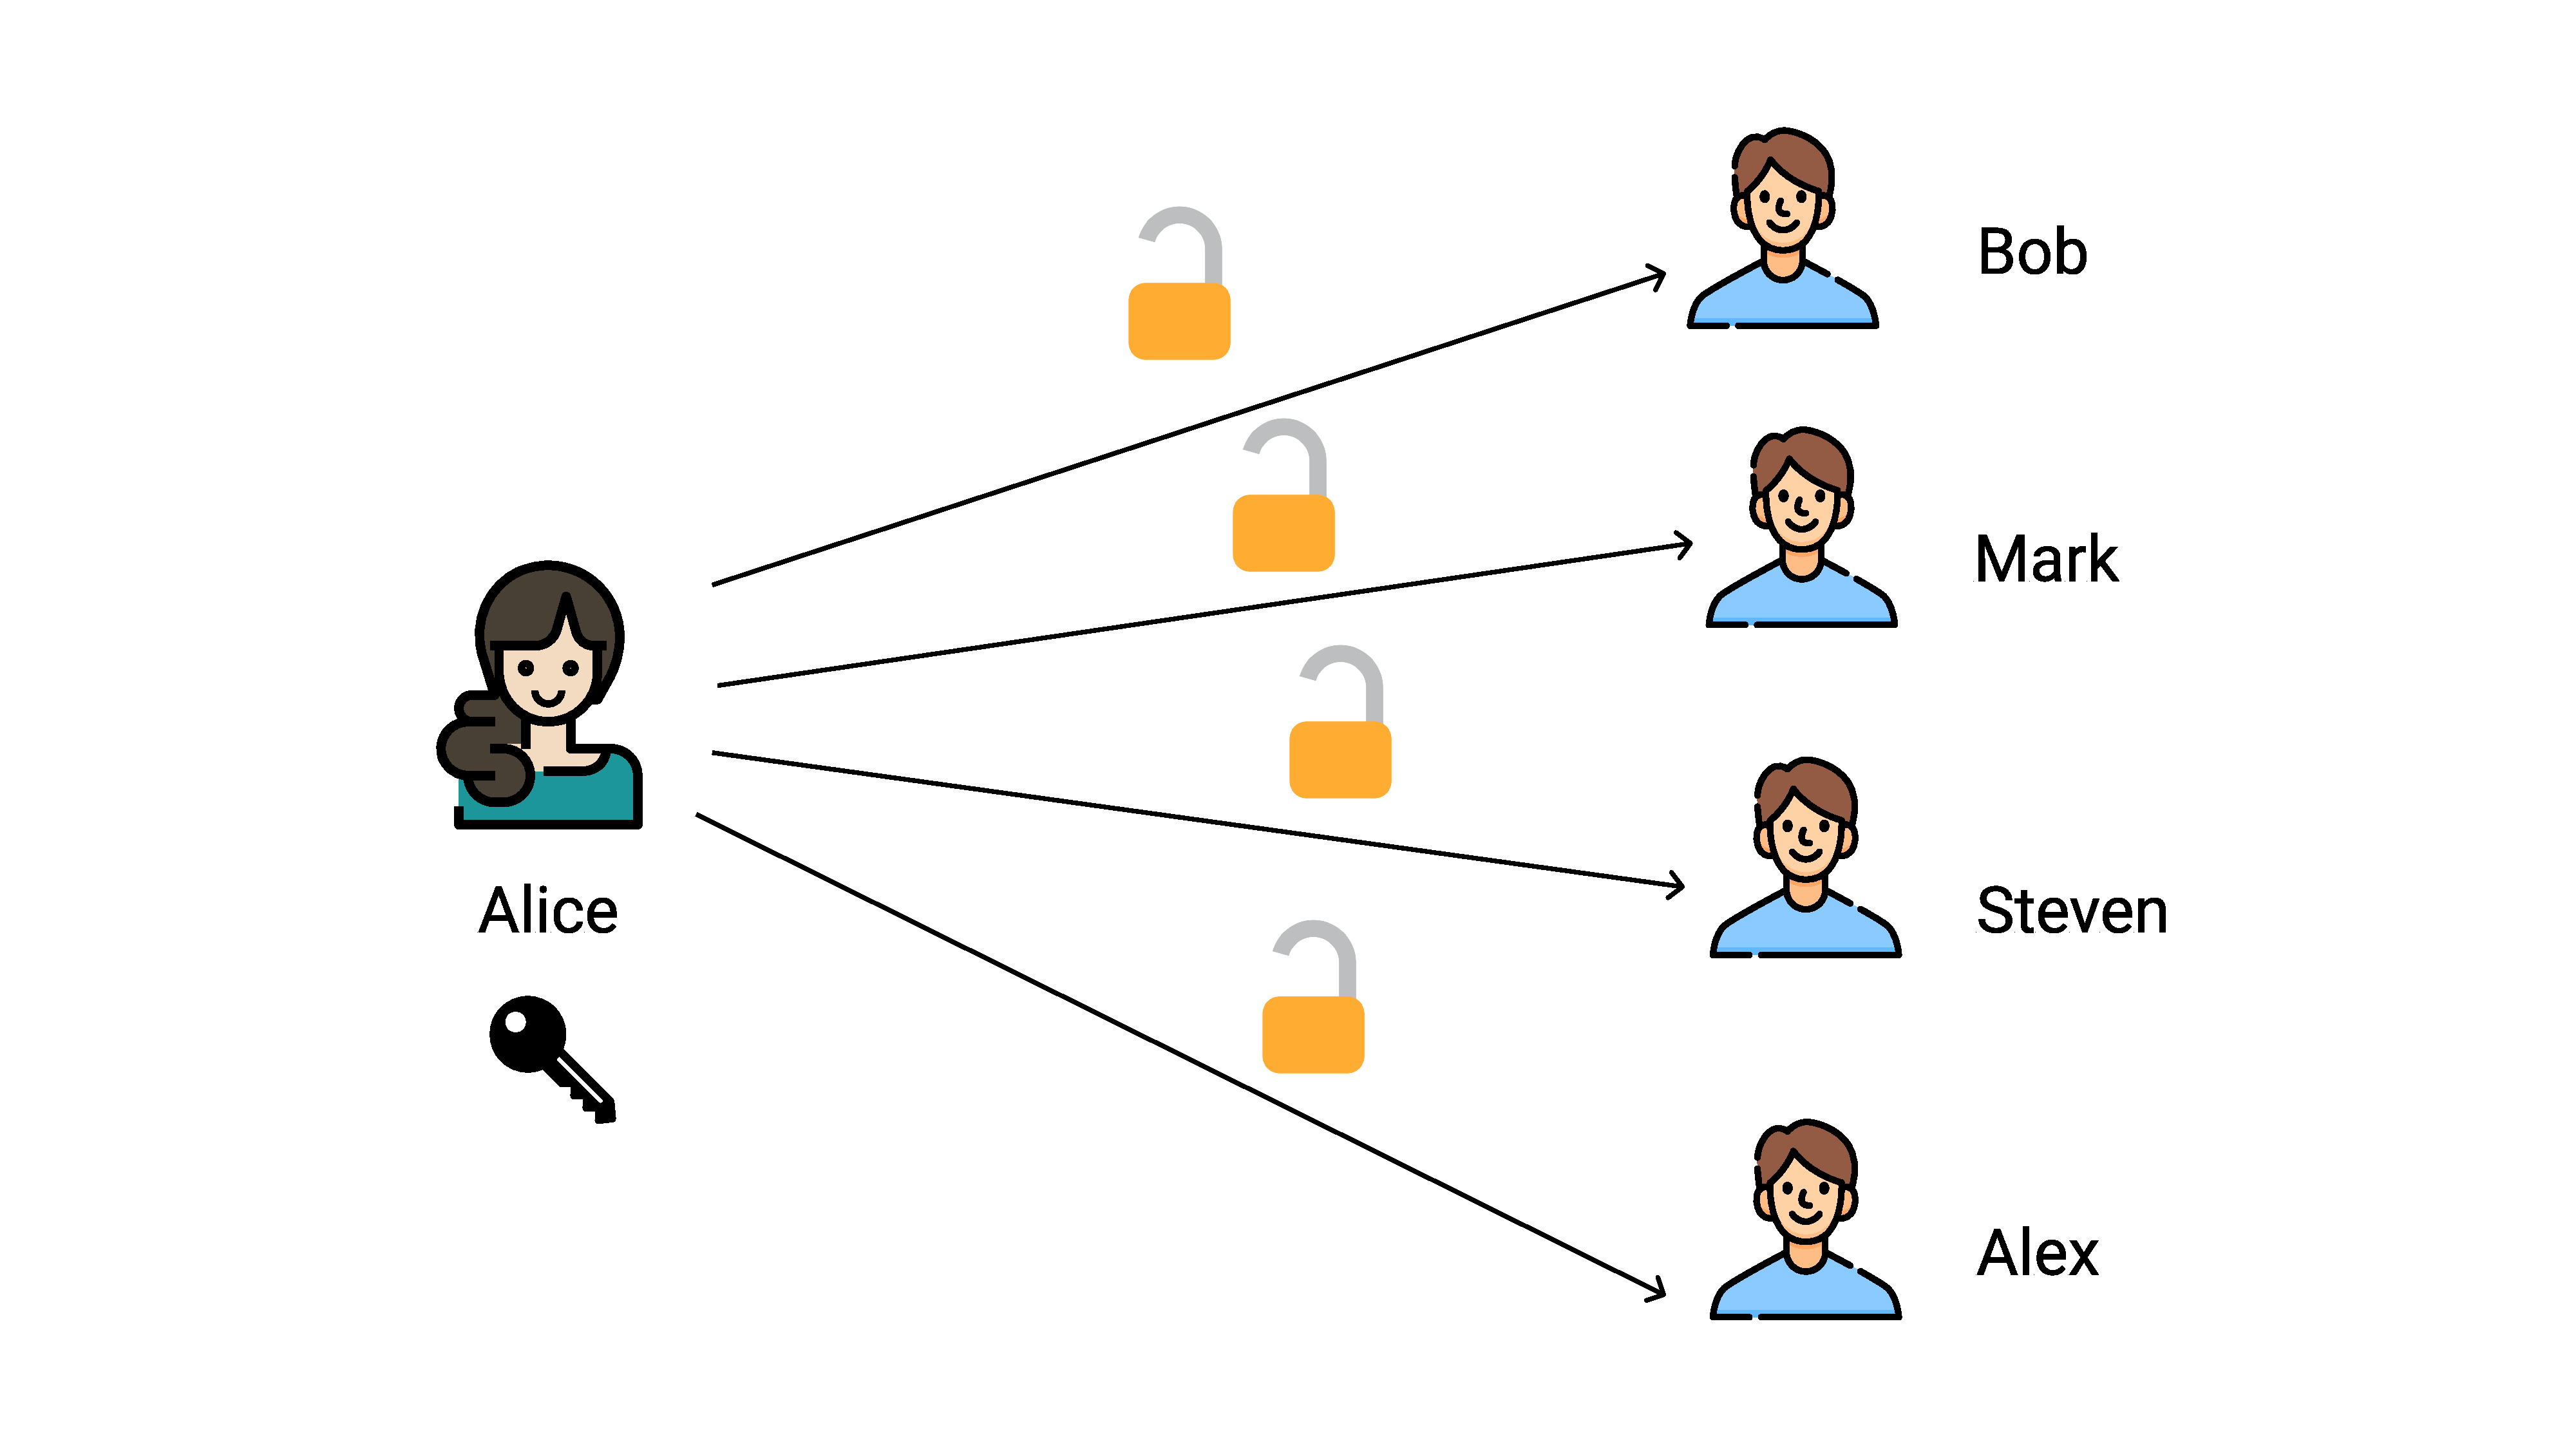
\includegraphics[width=1.15\textwidth]{img/Asymmetric_encryption}
    ~\caption{Asymmetric encryption real life example.} \label{fig:asymmetric-encryption}
\end{figure}
Therefore, the guys Bob, Mark, Steven and Alex have received an \textbf{opened lock} or \textbf{public key} from Alice.
Now all of them is can send a secret encrypted message to Alice simply putting it to the chest closing by the lock (public key)
received from Alice so that only Alice can open it with her private key.
However, such a simple idea requires complex mathematical background.
A concept of opened lock may be interpreted in terms of one-way functions.
\begin{quote}
    \textbf{One-way function} -- is a function that is easy to compute on every input, but hard to invert given the output.
\end{quote}

\begin{figure}[H]
    \centering
    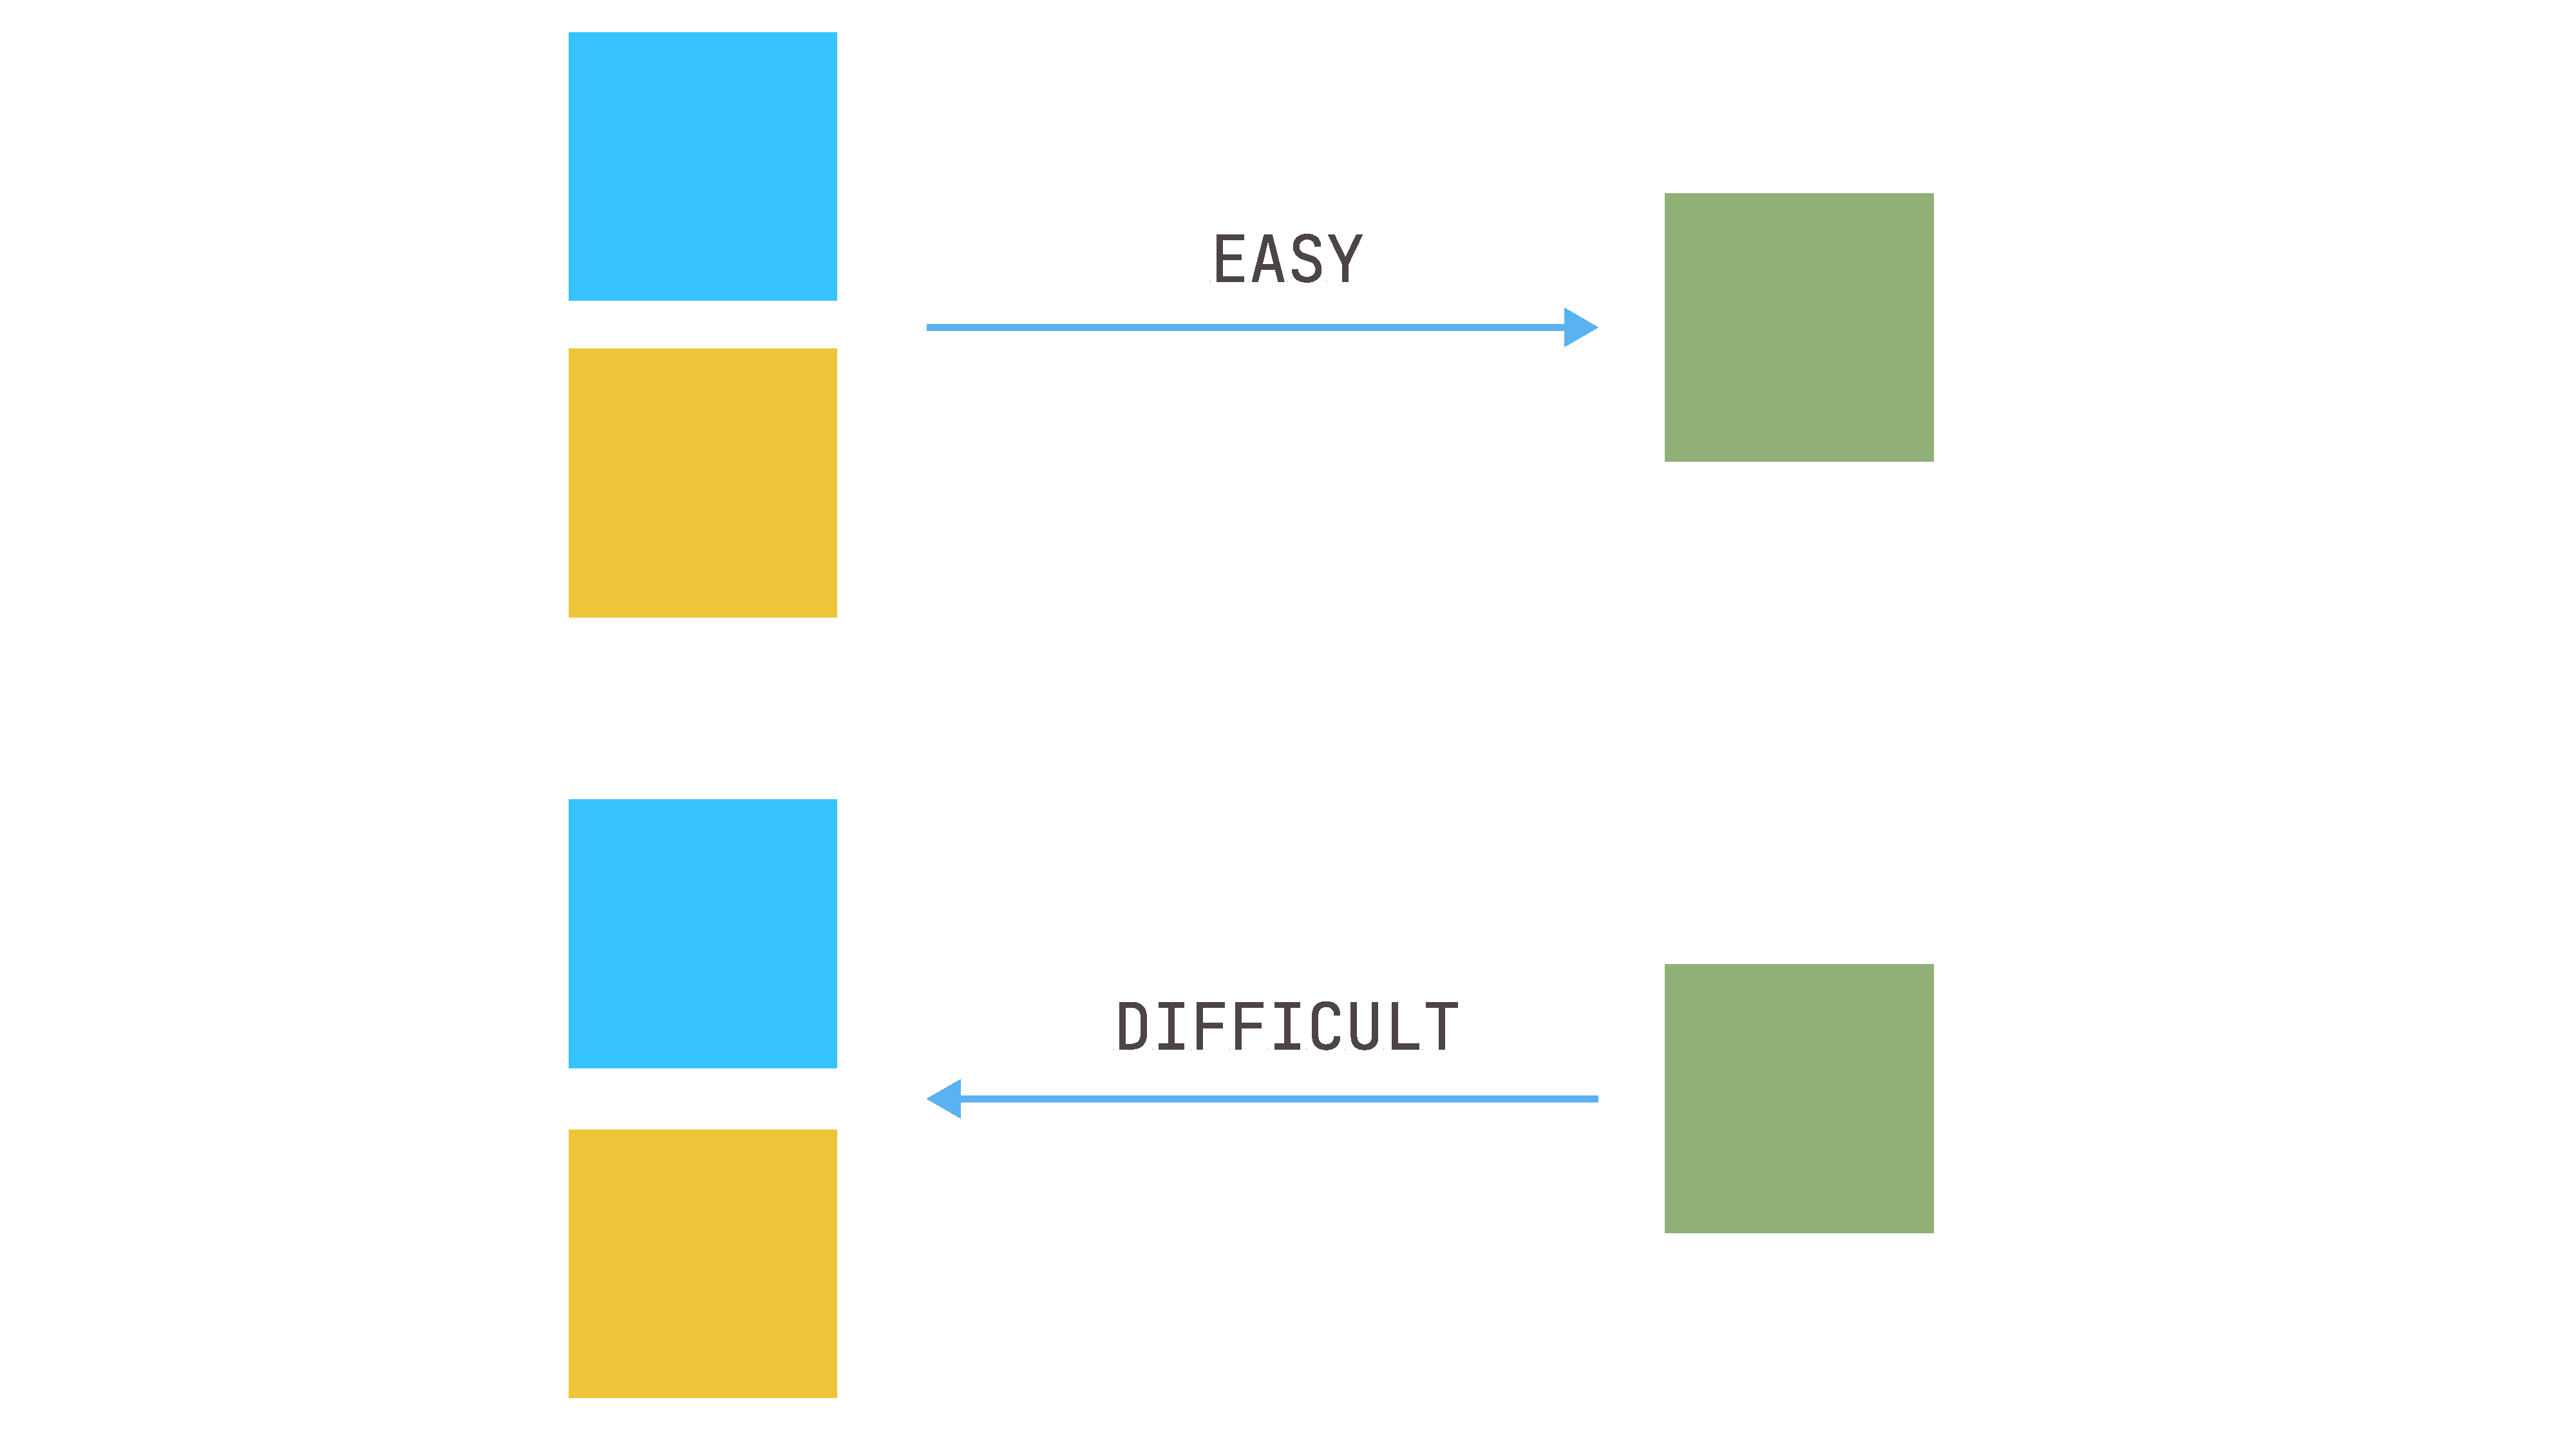
\includegraphics[width=1\textwidth]{img/One_Way_Functions}
    ~\caption{One-way function, analogy with paints}
    \label{fig:one-way-function}
\end{figure}
